\lab{Markov Chains}{Markov Chains}
\objective{Learn about Markov chains.}
\label{lab:EigSolve}

\section*{Markov chains}
A Markov chain is a collection of states with specified probabilities for transitioning from one state to another.
Markov chains are characterized by the fact that future behavior of the system depends only on its current state.

This lab is a very brief introduction to Markov chains. To learn more, see [TODO: ref something].

\subsection*{An example}
Suppose Fredo the frog is jumping between the three lily pads 1, 2, and 3.
These three pads are the \emph{possible states} of the system, and the lily pad on which Fredo is presently sitting is the \emph{current state}.
If Fredo is on lily pad 1 and jumps, there is a 25\% chance that it will land back on lily pad 1, a 25\% chance that it will land on lily pad 2, and a 50\% chance that it will land on lily pad 3.
These probabilities are the \emph{transition probabilities}.
Figure \ref{fig:markov1} is a \emph{transition diagram} that depicts all transition probabilities.

\begin{figure}
\begin{tikzpicture}[normalcircle/.style={draw, circle, minimum size=1cm, fill=shadecolor, thick, node distance=1.5cm} ]

\node[normalcircle](circle1)[]{};
\node[draw=none](one)[]{1};

\node[draw=none, node distance=2.5cm](dummy)
	[below of=circle1]{};

\node[normalcircle](circle2)[left of=dummy]{};
\node[draw=none, node distance= 1.5cm](two)[left 
	of=dummy]{2};
\node[normalcircle](circle3)[right of=dummy]{};
\node[draw=none, node distance= 1.5cm](three)
	[right of=dummy]{3};

\foreach \s /\t in {circle2/circle1, circle1/circle3, circle3/circle2}
	{\path[draw,bend left=20, thick, ->, >=stealth'] (\s)edge(\t);}
\foreach \s /\t in {circle1/circle2, circle3/circle1, circle2/circle3}
	{\path[draw,bend left=20, thick, ->, >=stealth'] (\s)edge(\t);}

\draw[thick,->, >=stealth'](-1.9,-2.8) arc (325:40:.4 and .5); 
\draw[thick,->, >=stealth'](1.9,-2.2) arc (500:215:.4 and .5); 
\draw[thick,->, >=stealth'](-.4,.3) arc (220:-35:.5 and .4); 

\node[draw=none, node distance=1.6cm](dummy2)
	[below of=circle1]{};
\node[draw= none, node distance=.3cm](midvalues)
	[above left of=dummy2]{$\frac{1}{4}$};
\node[draw= none, node distance=.3cm](midvalues2)
	[above right of=dummy2]{$\frac{1}{2}$};
\node[draw= none, node distance=.25cm](midvalues3)
	[below of=dummy2]{$\frac{1}{3}$};
\node[draw=none, node distance=1.6cm](outsidevalue)
	[above left of=midvalues3]{$\frac{1}{2}$};
\node[draw=none, node distance=1.6cm](outsidevalue2)
	[above right of=midvalues3]{$\frac{1}{2}$};
\node[draw=none, node distance=1.35cm](outsidevalue3)
	[below of=midvalues3]{$\frac{1}{2}$};
\node[draw=none, node distance=1.25cm](circlevalue)
	[above of=circle1]{$\frac{1}{4}$};
\node[draw=none, node distance=2.8cm](circlevalue2)
	[left of=dummy]{$\frac{1}{6}$};
\node[draw=none, node distance=2.8cm](circlevalue3)
	[right of=dummy]{$0$};

\end{tikzpicture}
\caption{Transition diagram for Fredo the Frog.}
\label{fig:markov1}
\end{figure}

We can convert our transition diagram into a \emph{transition matrix} The $(i,j)$-entry of the transition matrix is the probability that Fredo jumps from lily pad $j$ to lily pad $i$.
Fredo's transition matrix is
\[
A = \begin{pmatrix}
1/4 & 1/2 & 1/2\\
1/4 & 1/6 & 1/2\\
1/2 & 1/3 & 0
\end{pmatrix}.
\]

At any time, the chances that Fredo is on each lily pad is encoded by a \emph{state distribution vector} $\x = (x_1, x_2, x_3)^T$, where $x_i$ is the probability that Fredo is on lily pad $i$. 
For $\x$ to be a state distribution vector, we require $x_i\geq 0$ and $\|\x\|_1=1$ (recall that the 1-norm of a column vector is the sum of the magnitudes of its entries). 
Then $A\x$ will be another state distribution vector, which tells us the probability that Fredo is on each lily pad after one jump.

Thus, we can use Fredo's transition matrix to find where he will be after $k$ jumps. In fact, the $(i,j)$-entry of $A^k$ is the probability that Fredo goes from lily pad $j$ to lily pad $i$ in $k$ jumps. 
In our case,

\[
A^2 \approx \begin{pmatrix}
0.4375 & 0.3750 & 0.3750\\
0.3542 & 0.3194 & 0.2083\\
0.2083 & 0.3056 & 0.4167
\end{pmatrix}.
\]
Therefore, if Fredo starts on lily pad 1, there is a 43.75\% chance it will still be on lily pad 1 after two jumps.
Maybe Fredo jumped from 1 to 1 to 1, denoted $1 \rightarrow 1 \rightarrow 1$, or perhaps it jumped to one of the other lily pads and then back again, that is, either $1 \rightarrow 2 \rightarrow 1$ or $1 \rightarrow 3 \rightarrow 1$.

In addition, there is a 35.42\% chance Fredo will be on lily pad 2 and a 20.83\% chance that it will be on lily pad 3.
We can type our transition matrix into Python and see where Fredo is likely to be after any number of jumps.

\begin{lstlisting}
# The 1.'s in the numerator force floating point division.
>>> A = np.array([[1./4,1./2,1./2],[1./4,1./6,1./2],[1./2,1./3,0]])
>>> np.linalg.matrix_power(A,10)
array([[ 0.40000057,  0.39999962,  0.39999962],
       [ 0.30002369,  0.29999268,  0.29997574],
       [ 0.29997574,  0.3000077 ,  0.30002464]])
\end{lstlisting}

In fact, as we take higher and higher powers of $A$, it appears that 
\[
\lim_{k \rightarrow \infty} A^k = \begin{pmatrix}
0.4 & 0.4 & 0.4\\
0.3 & 0.3 & 0.3\\
0.3 & 0.3 & 0.3
\end{pmatrix}.
\]
This means that Fredo's state distribution approaches $(0.4, 0.3, 0.3)^T$ after many jumps, regardless of his initial state distribution.

Moreover, suppose Fredo's initial state distribution is $(0.4, 0.3, 0.3)^T$. 
We can use Python to compute his state distribution after 1 jump.
\begin{lstlisting}
>>> A.dot(np.array([0.4,0.3,0.3]))
array([ 0.4,  0.3,  0.3])
\end{lstlisting} 
Fredo's state distribution after a jump stays ``fixed.'' We call the vector $(0.4, 0.3, 0.3)^T$ a \emph{stable fixed point} for Fredo.


\subsection*{General Markov chains}
Let us generalize this example. A Markov chain is a collection of states with the probabilities that we will move from one state to another. 
These transition probabilities are encoded in a transition matrix, whose $(i-j)$-entry is the probability of moving from state $j$ to state $i$. 
Each column of such a matrix will necessarily have entries that sum to 1. 

%When we have a Markov chain, we want to know what the state distribution is after our system has been running for some time. We are especially interested if the state distributions converge to something that is independent of the initial state, as was the case for Fredo. That is, we want to know about stable fixed points.

Let $A$ be the transition matrix of a Markov chain. 
Then a state distribution vector $\x$ is a \emph{stable fixed point} if $A\x=\x$. 
So $\x$ is a stable fixed point if and only if $\x$ is a positive unit eigenvector of $A$ corresponding to the eigenvalue 1. 


Every Markov chain has at least one stable fixed point. 
If in addition we assume some power $A^k$ of $A$ has all positive (nonzero) entries, then the stable fixed point is unique. 
In this case, $A^k$ will converge to a matrix whose columns are all equal to the unique stable fixed point.

Note that Fredo's transition matrix does not have positive entries, but its square does. 
So Fredo has the unique stable fixed point $(0.4, 0.3, 0.3)^T$.

\subsection*{Finding stable fixed points}
Calculating stable fixed points is an important problem in Markov chain analysis. 
Suppose a Markov chain has a transition matrix $A$ such that $A^k$ has strictly positive entries for some $k$. 
Then the \emph{Perron-Frobenius theorem} says that 1 is the unique eigenvalue of $A$ of largest magnitude, and the corresponding eigenvector is unique. 
This means that we can use the power method to find the unique stable fixed point of $A$.

Let us look at what the power method is doing in the example of Fredo the frog. 
We will use the 1-norm. 

Suppose we know Fredo starts on lily pad 1. Then we begin with the state distribution vector
\[
\x_0 = \begin{bmatrix}
1\\
0\\
0
\end{bmatrix}
\]
because we know for certainty (100\%) that Fredo is in the first state.
The next iteration of the power method is $\x_1=A\x_0/\|A\x_0\|_1$. But since $\|A\x_0\|_1=1$, this is just
\[
\x_1 = A \x_0 = \begin{bmatrix}
0.25\\
0.25\\
0.50
\end{bmatrix},
\]
which is exactly Fredo's state distribution after 1 jump.
After two jumps, Fredo's state distribution is
\[
\x_2 = A \x_1 = A^2 \x_0 = \begin{bmatrix}
0.4375\\
0.3542\\
0.2083
\end{bmatrix},
\]
which is also the second iteration of the power method.
After a large number of jumps, we have
\[
\x_n = A \x_{n-1} = \dots = A^n \x_0 \approx \begin{bmatrix}
0.4\\
0.3\\
0.3
\end{bmatrix}.
\]
Thus, the limiting vector of the power method is exactly the unique stable fixed point of the Markov chain. 

\subsection*{A final example}
Consider the Markov chain with transition matrix
\[
A = \begin{pmatrix}
0.5 & 0.3 & 0.4\\
0.2 & 0.2 & 0.3\\
0.3 & 0.5 & 0.3
\end{pmatrix}.
\]

Because all entries of $A$ are positive, the Markov chain has a unique stable fixed point. 
We could find this fixed point with the power method as outlined above, or we can do it by computing eigenvalues and eigenvectors in Python, as shown below.
\begin{lstlisting}
>>> from scipy import linalg as la
>>> A = np.array([[.5,.3,.4],[.2,.2,.3],[.3,.5,.3]])
>>> evals, evecs = la.eig(A)
>>> evals
array([ 1.        ,  0.14142136, -0.14142136])
\end{lstlisting}
We are interested in the eigenvalue 1, which is the first one outputted in this case. 
The corresponding eigenvector is the first column of \li{evecs}; let us call it \li{x}.
\begin{lstlisting}
>>> x = evecs[:,0]
\end{lstlisting}
Now, the one-norm of \li{x} will probably not be 1. To make it 1, we divide by the one-norm of \li{x}.
\begin{lstlisting}
>>>x = x/np.sum(x)
\end{lstlisting}
Finally, let us check that \li{x} is a stable fixed point of $A$. There are two things to check.
\begin{lstlisting}
# Check Ax = x
>>> np.allclose(A.dot(x),  x)
True

# Check ||x||_1 = 1
>>> np.sum(x)==1
True
\end{lstlisting}

\begin{problem}
Write a function that accepts as input a transition matrix, a vector representing the initial state, and a number of iterations \li{niter}. Your function should
\begin{enumerate}
\item Assume that the input matrix has a unique stable fixed point.
\item Calculate the unique stable fixed point by computing eigenvectors and eigenvalues in Python.
\item Return the current state of the Markov chain after \li{niter} iterations and the stable fixed point.
\end{enumerate}
\label{prob:markov}
\end{problem}

\begin{problem}
Suppose a basketball player's success at shooting free throws can be described with the following Markov chain
\[
A = \begin{pmatrix}.75&.50\\.25&.50\end{pmatrix}
\]
where the first state corresponds to success and the second state to failure. Use the function you wrote in Problem \ref{prob:markov} to answer the following questions.
\begin{enumerate}
\item If the player makes his first free throw, what is the probability that he also makes his third one? 
(That is, what is the probability that this system starts in state 1 and is still in state 1 after 3 steps?)
\item What is the player's average free throw percentage? 
(This is equal to the success-component of the stable fixed point.)
\end{enumerate}
\label{prob:markov_freethrow}
\end{problem}

\begin{comment}
\begin{problem}
Consider the Markov process given by the transition diagram in Figure \ref{fig:markov2}.
\begin{figure}[H]
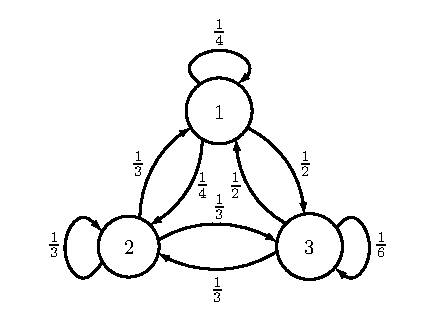
\includegraphics[width=\textwidth]{markov2}
\caption{Transition diagram}
\label{fig:markov2}
\end{figure}

\begin{enumerate}
\item Find the transition matrix.
\item If the Markov process is in state 1 initially, find the probability that it is in state 2 after two transitions.
\item Find the stable fixed point if it exists.
\end{enumerate}
\label{prob:markov_stablept}
\end{problem}
\end{comment}